\documentclass{letter}

\usepackage[left=0.75in, right=0.75in, top=1.1in, bottom=0.75in]{geometry}
\usepackage{fancyhdr, amsmath, amssymb, mathtools, xcolor, graphicx, listings, mathpazo}
\graphicspath{{.}}

\pagestyle{fancy}
\fancyhf{}
\rhead{Page \thepage}
\chead{AMSC808N Final Exam Problem 1}
\lhead{Tyler Hoffman}
\setlength{\headsep}{0.2in}

\newcounter{problem}
\newcounter{subproblem}[problem]
\newcounter{solution}

\renewcommand{\thesubproblem}{(\alph{subproblem})}

\newcommand{\Problem}[2]{%
	\stepcounter{problem}%
	\leftskip=0pt%
	\theproblem.~\textbf{{#1.}} #2 \par%
}

\newcommand{\Subproblem}[1]{%
	\stepcounter{subproblem}%
	\leftskip=15pt%
	\thesubproblem~ #1 \par%
}

\newcommand{\Solution}[1]{%
	\textbf{Solution.} #1 \par%
}

\newcommand{\Due}[1]{\textbf{Due: #1} \par}

\newcommand{\UNFINISHED}{\textbf{\color{red} UNFINISHED}}
\newcommand{\CHECK}{\textbf{\color{orange} CHECK ME}}

\newcommand{\iu}{{i\mkern1mu}}
\newcommand{\T}{\intercal}
\newcommand{\R}{\mathbb{R}}
\newcommand{\relu}{\mathrm{ReLU}}

\DeclareMathOperator{\diag}{diag}
\DeclareMathOperator{\rank}{rank}
\DeclareMathOperator{\nul}{nul}
\DeclareMathOperator{\tr}{tr}

\usepackage{hyperref}
\begin{document}
    \Due{21 Dec 2020}

    The code for this problem can be found at \href{https://github.com/thoffman1/amsc808n/tree/master/final/problem1}{this Github link}.

    Suppose we want to approximate the function $g(x) = 1 - \cos(x)$ on the interval $[0, \pi/2]$ with the function $\relu(ax - b)$ where $a$ and $b$ are to be determined. We take 6 training points $x_j = \pi j/10$, $j = 0,1,2,3,4,5$ and set up the following loss function: \begin{align*}
        f(a, b) = \frac{1}{12}\sum_{j = 0}^5 [\relu(ax_j - b) - g(x_j)]^2.
    \end{align*}

    \Problem{Stationary points}{The set of stationary points of $f$ (i.e., the set of points where $\nabla f = 0$) consists of the global minimizer and a flat region. Describe this set analytically using equalities and inequalities and show it in a figure. Provide an analytic formula for the global minimizer of $f$. What is the global minimum of $f$?}
    \Solution{To begin, we compute the partial derivatives of $f$. \begin{align*}
        \frac{\partial f}{\partial a} &= \frac{1}{6}\sum_{j = 0}^5 x_j[\relu(ax_j - b) - g(x_j)]\relu'(ax_j - b) \\
        \frac{\partial f}{\partial b} &= -\frac{1}{6}\sum_{j = 0}^5 [\relu(ax_j - b) - g(x_j)]\relu'(ax_j - b)
    \end{align*} where the derivative of the $\relu$ is defined as \begin{align*}
        \relu'(x) = \begin{cases} 1 & x > 0 \\ 0 & x < 0. \end{cases}
    \end{align*} In order to guarantee that the partials are equal to 0, we look for values of $a$ and $b$ that make the terms in the interior equal to 0. First, we study the $\relu'$ factor and notice that \begin{align*}
        \relu'(ax_j - b) = 0 \iff ax_j - b < 0
    \end{align*} so $b > ax_j$ for all $j$ in order to zero out every term in both sums. Since $x_0 = 0$, we know $b > 0$. When $a > 0$, we need $b > \max_j ax_j = \frac{\pi}{2}a$ and when $a < 0$, we need $b > \min_j ax_j = 0$ since the inequality flips when $a < 0$. Naturally, when $a = 0$ we simply need $b > 0$ (as $\relu(-b) = 0$ for $b > 0$), which squares up with the above characterization. This flat region can be seen in Figure 1 below. To find the minimizer, \UNFINISHED

    \begin{center}
        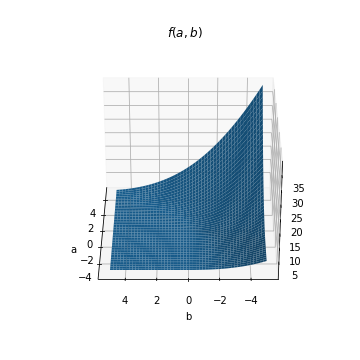
\includegraphics[trim={1cm 1cm 1cm 0cm},clip,scale=0.7]{../pics/loss_surface.png} 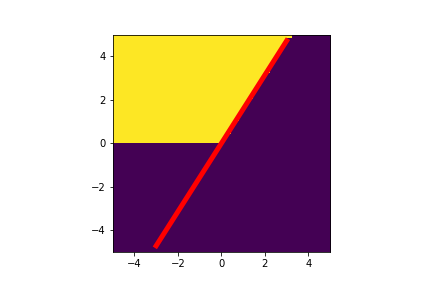
\includegraphics[trim={1cm 0cm 1cm 0cm},clip,scale=0.7]{../pics/flat_region.png}\\
        Figure 1: Left: surface of $f(a, b)$ near the origin. Right: flat region $\nabla f = 0$. The yellow region is the flat region, the purple region is the rest of the function, and the red line is the boundary $b = \frac{\pi}{2}a$.
    \end{center}}

    \Problem{Gradient descent}{Take $a = 1$ and $b = 0$ as the initial guess for gradient descent with constant stepsize. What is the minimal stepsize $\alpha^*$ such that the iterates end up in the flat region? Suppose we take $\alpha = 0.99\alpha^*$ and run gradient descent. Will the iterates approach the global minimizer? Either way, explain why. Propose a stepsize trying to make it as large as possible such that the iterates will necessarily converge to the global minimizer and give a rationale for your choice.}
    \Solution{The gradient descent iteration is $x_{k+1} = x_k - \alpha \nabla f(x_k)$. Here, $x = [a, b]^\T \in \R^2$.\UNFINISHED}

    \Problem{Stochastic gradient descent}{As above, take $a = 1$ and $b = 0$ as the initial guess. Use a simple stochastic gradient descent with a single training point chosen randomly for approximating the gradient of $f$ at each step. Find a strategy for stepsize reduction such that the stochastic gradient descent will converge to the global minimizer.}
    \Solution{See \texttt{prob1.ipynb} for my stochastic gradient descent code. I tested the following schedules: \begin{itemize}
        \item Reciprocal: $\alpha_k = L/k$
        \item Power: $\alpha_k = L2^{-k-1}$
        \item Exponential $\alpha_k = Le^{-rk}$ where $r$ controls the speed of the decay
        \item Drop: $\alpha_k = Lr^{\lfloor k/M \rfloor}$ where $M$ is the number of steps we take per drop
    \end{itemize} In all of these, $L$ is a constant initial learning rate. These all satisfy $\sum_{k=0}^\infty \alpha_k = \infty$, $\sum_{k=0}^\infty \alpha_k^2 < \infty$. \UNFINISHED}
\end{document}